\documentclass[12pt]{aghdpl}
% \documentclass[language=en,11pt]{aghdpl}  % praca w języku angielskim
\usepackage{listings}
\usepackage{multirow}
\usepackage{hyperref}
\hypersetup{
    colorlinks=true,
    linkcolor=black,
    filecolor=black,      
    urlcolor=black,
    pdftitle={Sterowany mową interfejs człowiek-maszyna},
    pdfpagemode=FullScreen,
    }
%---------------------------------------------------------------------------

\author{Kamila Kopacz}


\titlePL{Sterowany mową interfejs człowiek-maszyna }
\titleEN{Voice-Controlled Human Machine Interface System }

\thesistype{Projekt dyplomowy}

\supervisor{dr inż. Łukasz Więckowski}

\degreeprogramme{Automatyka i Robotyka}

\date{2024}

%\department{Katedra Informatyki Stosowanej}
%\department{Department of Applied Computer Science}

\faculty{Wydział Elektrotechniki, Automatyki, Informatyki i Inżynierii Biomedycznej}
%\faculty{Faculty of Electrical Engineering, Automatics, Computer Science and Biomedical Engineering}

\acknowledgements{Serdecznie dziękuję moim przyjaciołom za to, że są.}


\begin{document}

	\titlepages
	\RedefinePlainStyle
	
	\setcounter{tocdepth}{2}
	\tableofcontents
	\clearpage
	
	\chapter{Wstęp}
\label{cha:Wstęp}

Celem projektu jest wykonanie i przetestowanie nowego interfejsu człowiek-maszyna, który wykorzysta jeden z dostępnych algorytmów rozpoznawania języka naturalnego.

We współczesnym świecie można znaleźć wiele przykładów sterowania maszynami. Jedną z nich jest między innymi łazik planetarny Kalman, projekt rozwijany przez członków koła naukowego AGH Space Systems.  Sterowanie poruszaniem się tego robota możliwe jest poprzez wykorzystanie skonstruowanego przez studentów urządzenia \cite{jklazik}. Za pomocą odpowiednich przycisków i gałek uruchamiane są odpowiadające im części napędu jezdnego. Innowacyjna konstrukcja tego urządzenia i modernizacja sposobu sterowania robotem, który z naciskania przycisków na klawiaturze laptopa przerodził się w osobny moduł jedynie podłączany kablem nasuwa sugestię możliwości pójścia o krok dalej.

Co gdyby algorytm sterowania maszyną został przeniesiony z powrotem do komputera, ale pozbawiony potrzeby wchodzenia w kontakt fizyczny poprzez umożliwienie sterowania głosowego? Jest to pytanie na które odpowiedź jest stawiana w wielu dziedzinach życia codziennego, zaczynając od asystentów obecnych w każdym smartfonie, poprzez obsługiwanie funkcji w samochodach, a kończąc na aktywacji urządzeń przemysłowych. Jest to nie tylko funkcjonalność przydatna w momencie, kiedy osoba obsługująca daną maszynę nie ma możliwości wykonania danej czynności własnoręcznie. Dla osób niepełnosprawnych, posiadających ograniczenia ruchowe, jest to niejednokrotnie umożliwienie używania danego urządzenia i poszerzenie zakresu dostępności.

Jak wiele nowatorskich dziedzin rozwoju, również i ta technologia wymaga pracy nad nią i ciągłego dostosowywania jej do codziennych potrzeb. Biorąc na przykład asystenta głosowego Google, dostępnego w większości telefonów komórkowych z Androidem, już po krótkim czasie używania można zauważyć występujące czasem nieścisłości w rozpoznawaniu i rozumieniu przez aplikację danej wypowiedzi. Jest to bezpośrednio powiązane z zastosowanymi algorytmami rozpoznawania głosowego, które inaczej niż człowiek, nie zawsze są w stanie poprawnie zinterpretować ludzką mowę. 

Praca dyplomowa obejmie przegląd istniejących możliwości sterowania głosowego urządzeniami. Zaprezentowana zostanie analiza wykorzystywanych w prototypowych aplikacjach modeli uczenia maszynowego, a na jej podstawie napisany algorytm służący do sterowania głosowego. Poprawność implementacji zweryfikuje podłączenie algorytmu w środowisku Robot Operating System do symulacji przykładowego robota w programie Gazebo. Następnie przy użyciu biblioteki Custom Tkinter zostanie wykonany interfejs służący do sterowania robotem.


%---------------------------------------------------------------------------

\section{Rozpoznawanie głosowe}
\label{sec:rozpoznawanieGlosowe}

Rozpoznawanie głosu to umiejętność wykonywania przez urządzenie identyfikacji zadanych mu komend. Dzieje się to poprzez wykorzystanie konwersji A/D do przetworzenia sygnału analogowego w cyfrowy (Rys.\ref{fig:ad}). 

\begin{figure}[h]
    \centering
    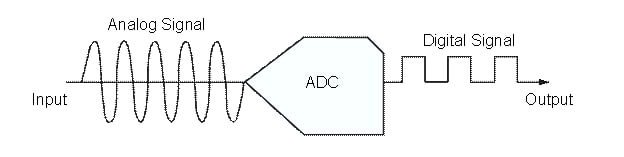
\includegraphics{files/ad.jpg}
    \caption{Konwersja A/D. (Źródło: \url{https://wiki.analog.com/university/courses/electronics/text/chapter-20})}
    \label{fig:ad}
\end{figure}

Komputer do rozszyfrowania sygnału cyfrowego, musi posiadać bazę słów i sylab do porównywania ich do siebie. W rzeczywistości, aby algorytm służący do rozpoznawania głosu był w stanie poprawnie przetworzyć zadaną mu komendę, potrzebuje sporej ilości pamięci RAM, aby wystarczająco szybko znaleźć odpowiadający sygnałowi cyfrowemu wzorzec. Analizowana jest nie tylko sama treść, ale również częstotliwość głosu, akcent czy poprawność wymowy. Ponadto, sygnał analogowy musi zostać wcześniej przeprocesowany, celem pozbycia się szumów lub dźwięku w tle.

Technologie służące rozpoznawaniu głosu przebyły długą drogę aby znaleźć się we współczesności. Idea stworzenia urządzenia, które jest w stanie rozpoznawać mowę i przetwarzać ją na tekst narodziła się z prostej ludzkiej chęci to usprawniania powtarzających się zadań. Już w XIX wieku powstało pierwsze urządzenie rejestrujące dźwięk, które niedługo później przerodziło się w znany nam obecnie dyktafon, a zapoczątkowało falę mechanizacji pracy biurowej. Wprowadzone w życie codzienne zostały między innymi maszyny do pisania, które swoją przydatnością wpłynęły na wytworzenie się konceptu aktywowanej głosowo maszyny do pisania. 

Próby wytworzenia urządzenia zdolnego do automatycznego rozpoznawania głosu były w większości oparte na podstawowych elementach fonetycznych języka i tego jaki jest proces ich tworzenia. Aby wyprodukować dźwięk samogłoski, struny głosowe muszą odpowiednio wibrować, aby powietrze które przepływa przez nie uzyskało odpowiednią częstotliwość. Fakt ten został wykorzystany w 1952 roku, kiedy to Davis, Biddulph, i Balashek z Bell Laboratories stworzyli pierwszy system do rozpoznawania głosowego, zdolny do interpretacji cyfr mówionych przez jednego z twórców. Na podstawie wartości pasm częstotliwości dźwięku każdej samogłoski powstał wzór dla maszyny, z którego mogła ona odczytać region występowania częstotliwości dla każdej z cyfr. Następnie odnosząc się do posiadanego wzoru mogła ona zidentyfikować daną cyfrę \cite{juang2005automatic}.

Współczesne urządzenia posiadające funkcję rozpoznawania głosowego zawierają w sobie nie tylko odpowiednie elementy mechaniczne i elektroniczne. Na możliwość wykonywania tej czynności składają się algorytmy uczenia maszynowego i sieci neuronowe. Z najbardziej rozpoznawalnych i ogólnie dostępnych na rynku zastosowań można wyróżnić między innymi elementy \textit{smart home} takie jak Apple HomeKit, Amazon Alexa czy dostępny w wielu smartfonach Google Assistant.


%---------------------------------------------------------------------------

\section{Przetwarzanie języka naturalnego}
\label{sec:przetwarzanieJezykaNaturalnego}

Natural Language Processing (NLP) jest to dziedzina sztucznej inteligencji zajmująca się szeroko pojętą komunikacją pomiędzy człowiekiem a maszyną. Jednym ze sposobów, w jaki można skategoryzować język, służący do takiej właśnie komunikacji, jest podział na \textit{naturalny} oraz \textit{nienaturalny}. Część naturalna odnosi się do wymiany informacji pomiędzy człowiekiem a robotem w sposób najbardziej zbliżony do komunikacji pomiędzy ludźmi, za pomocą słów złożonych w zdania o zadanym kontekście. Język \textit{nienaturalny} natomiast opisuje obszar komunikacji, w którym można zawrzeć między innymi języki programowania czy funkcjonalności pozwalające na obsługę maszyn w sposób dla nich domyślny, który od człowieka wymaga wcześniejszego doświadczenia. 

Język \textit{naturalny} podzielić można na dwie kategorie komunikacji: niewerbalną i werbalną. Pierwsza z nich obejmuje każdy przekaz, jaki człowiek może nadać, nie używając do wykonania tej czynności języka mówionego. Może być to ton głosu, postawa, gestykulacja, mimika twarzy, ale również dystans między rozmówcami, styl ubioru czy czas oraz miejsce konwersacji. Komunikacja niewerbalna niejednokrotnie niesie za sobą znaczenie przekazu, na które odbiorca może zareagować w określony dla danej sytuacji sposób. 

Komunikację werbalną, która opiera się na języku mówionym, w przetwarzaniu języka naturalnego można zobrazować jako widoczny na Rys.\ref{fig:nlp} proces przetwarzania dźwięku wydanego przez człowieka na wyrazy, a następnego ekstrakcję znaczenia i informacji z przekazu.

\begin{center}
    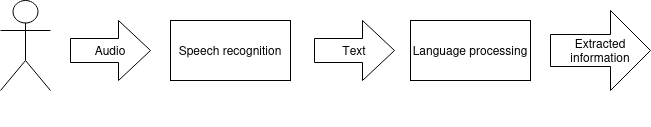
\includegraphics[width=12cm]{files/nlp.png}
    \captionof{figure}{Przetwarzanie języka naturalnego.}
    \label{fig:nlp}
\end{center}

%---------------------------------------------------------------------------

\subsection{Symboliczne przetwarzanie języka naturalnego}
\label{subsec:symbolic}

Do procesu przetwarzania języka naturalnego można podejść na wiele sposobów. Głównymi rozwiązaniami są systemy oparte na zestawie reguł i zasad (Symbolic NLP), oparte na prawdopodobieństwie (Statistical NLP) i oparte na sieciach neuronowych (Neural NLP). Pierwsze z nich do poprawnego działania wymagają stworzonej manualnie, obszernej bazy wiedzy, wykorzystywanej do ekstrakcji informacji, rozpoznawania konkretnych wzorców czy przeprowadzania klasyfikacji tekstu. 

Z uwagi na fakt, że język mówiony ciągle się zmienia, tj. tworzone są nowe zasady, formy gramatyczne oraz słowa, aby nadążyć za rozwojem ludzkości, implementacja wszystkich rządzących nim praw jest uciążliwa i czasochłonna. W związku z tym, systemy te często poza konkretnymi regułami, opierają się również na wykluczeniu niewystępujących naturalnie scenariuszy konwersacji. Bazując na tym systemie, proces przetwarzania przebiega następująco (Rys. \ref{fig:symbolic}): na podstawie charakterystyki danego zadania, tworzone są reguły spełniające założenia. Reguły te są iteracyjnie nakładane na dane wejściowe celem znalezienia istniejących wzorców i procesowane zgodnie z otrzymanymi rezultatami aby zwiększyć dokładność algorytmu. 

\begin{center}
    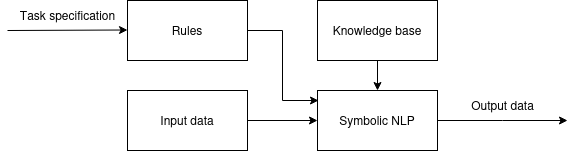
\includegraphics[width=12cm]{files/symbolic.png}
    \captionof{figure}{Symboliczne przetwarzanie języka naturalnego.}
    \label{fig:symbolic}
\end{center}

Pomimo tego, że systemy oparte na zestawie reguł i zasad są dokładne i rzetelne, jeśli zaimplementowane prawidłowo, aby były efektywne mogą być głównie stosowane do wykonywania mało złożonych zadań, ściśle określonych i z nałożonymi ograniczeniami. 

%---------------------------------------------------------------------------

\subsection{Statystyczne przetwarzanie języka naturalnego}
\label{subsec:statistyc}

W przypadku, gdy dane zadanie posiada wiele złożonych scenariuszy, stosowane są systemy oparte na prawdopodobieństwie, gdzie algorytm uczy się własnego działania na podstawie podanych mu wcześniej danych. Uczenie może przebiegać na jeden z trzech sposobów: 
\begin{itemize}
    \item uczenie nadzorowane (ang. supervised learning), gdzie model dostaje dane wejściowe oraz pożądane dane wyjściowe, a jego zadaniem jest znalezienie ścieżki pomiędzy nimi,
    \item uczenie nienadzorowane (ang. unsupervised learning), gdzie bazując tylko na danych wejściowych, model ma za zadanie wyciągnąć z nich informacje, 
    \item uczenie przez wzmacnianie (ang. reinforcement learning), gdzie zamiast podania modelowi danych, jest on umieszczany w środowisku, w którym poprzez automatyczne wyciąganie danych ma osiągnąć zadany cel. 
\end{itemize}

Na osiągnięte przez model rezultaty, wpływa nie tylko jakość danych, ale również sposób, w jaki informacje z nich są wyciągane. Podając algorytmowi do przetworzenia przykładowe zdanie, do wyciągnięcia informacji może on użyć \textit{kodowania 1 z n} (Rys. \ref{fig:one-hot}), gdzie w wektorze n-wymiarowym każdy element może mieć wartość 1 lub 0 w zależności czy w zdaniu o długości n występuje słowo istniejące w słowniku, czy nie. Do podejścia tego, można dołożyć częstość występowania słów, gdzie w wektorze odnoszącym się do danego słowa, zamiast 1 podana będzie jego liczność. 

\begin{center}
    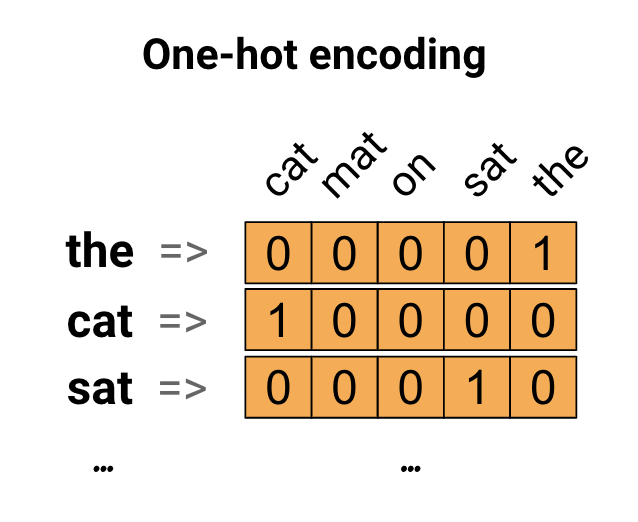
\includegraphics[width=10cm]{files/one-hot.png}
    \captionof{figure}{Kodowanie 1 z n. (Źródło: \url{https://www.tensorflow.org/text/guide/word_embeddings})}
    \label{fig:one-hot}
\end{center}

Nie tylko ze zdań można wyciągać informacje służące do przewidywania kolejnych elementów, ale również znaków czy sekwencji słów. Używając modeli \textit{n-gram}, które tworzą wektor wystąpień nie pojedynczego słowa, ale dwóch (bigrams) lub trzech (trigrams) (Rys.\ref{fig:n-gram}), można znacznie zwiększyć skuteczność modelu, ponieważ bierze on pod uwagę kontekst występowania słów w sekwencji. 
\begin{center}
    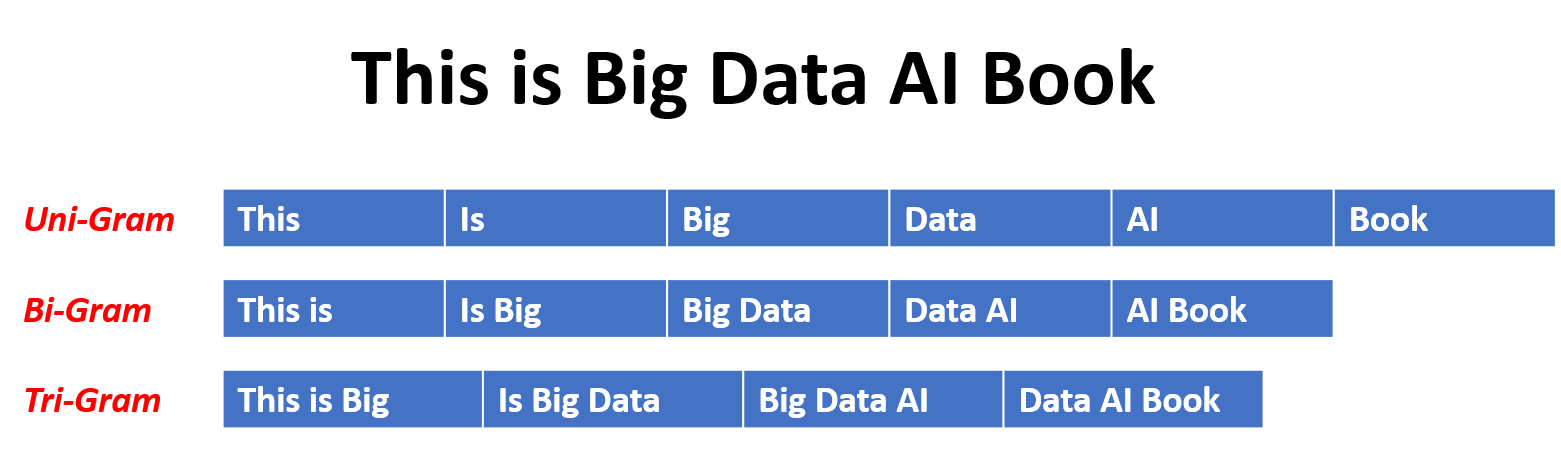
\includegraphics[width=10cm]{files/n-grams.png}
    \captionof{figure}{Unigram, bigram i trigram. (Źródło: \url{https://devopedia.org/n-gram-model#Mehmood-2019})}
    \label{fig:n-gram}
\end{center}

%---------------------------------------------------------------------------

\subsection{Neuronowe przetwarzanie języka naturalnego}
\label{subsec:neural}

Pomimo swojej szeroko pojętej użyteczności i zastosowań, nie wszystkie złożone problemy mogą zostać objęte podejściem statystycznym. Do wyciągnięcia niskopoziomowych właściwości tekstu czy radzenia sobie z długimi i skomplikowanymi danymi wejściowymi implementowane są sieci neuronowe. 

Używając uczenia nadzorowanego, wektory zawierające cechy każdego ze słów w danych wejściowych używane są do nauczenia modelu przewidywania następnych słów w podanym kontekście. Pojedyncze wykonanie tej czynności to \textit{warstwa} przez którą przechodzą dane w modelu. Warstwy te, nakładane na siebie tworzą właśnie sieci neuronowe. 

Współczesne systemy do rozpoznawania głosu bazują na ukrytym modelu Markova (hidden Markov model). Model ten opisuje obserwowalny proces (Rys. \ref{fig:markov}) A, którego rezultat zależy od rezultatu procesu E. Ponieważ stan E nie jest obserwowalny, jego stan może być znaleziony poprzez obserwację stanu A. Jest to adekwatne przedstawienie tego, czym jest proces występowania każdego po sobie wyrazu w zdaniu. Na podstawie ciągu składającego się ze znanego słowa i kolejnego, które wystąpi po nim, możliwe jest statystyczne przybliżenie wartości słowa nieznanego. Następnie w tym procesie sieci neuronowe rekurencyjnie używają danych wyjściowych z modelu dla poprzedniego kroku do wpłynięcia na dane wejściowe do kolejnego w sekwencji. 

\begin{center}
    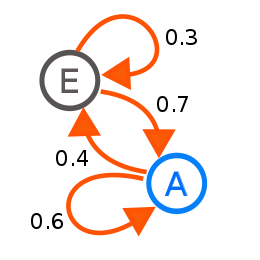
\includegraphics[width=10cm]{files/markov.png}
    \captionof{figure}{Diagram przedstawiający proces Markova. (Źródło: \url{https://commons.wikimedia.org/wiki/File:Markovkate_01.svg})}
    \label{fig:markov}
\end{center}

%---------------------------------------------------------------------------

	\chapter{Uczenie maszynowe}
\label{cha:uczenieMaszynowe}

Istnieje wiele metod, jakimi można podejść do zagadnienia rozpoznawania mowy. Spośród dostępnych otwartych (ang. open-source) oprogramowań wyróżnia się biblioteka \textit{SpeechRecognition} \cite{speechrec}, która umożliwia korzystanie z kilku popularniejszych Interfejsów Programistycznych Aplikacji (ang. API - Application Programming Interface) do rozpoznawania głosowego, w tym Google Web Speech API \cite{webspeech}. 

%---------------------------------------------------------------------------

\section{Środowisko zdalne}
\label{sec:srodZdal}

Używając biblioteki \textit{SpeechRecognition} możliwe jest zarówno rozpoznawanie mowy na podstawie nagrania \ref{fig:record} oraz odczytu z mikrofonu \ref{fig:microphone}. Przykłady połączenia jej on-line z zewnętrznym API, gdzie jako dane wejściowe zostało użyte nagranie oraz wypowiedzenie tej samej kwestii "go forward", znajdują się poniżej.

Poprzez stworzenie nowej instancji \textit{Recognizer}, funkcja \textit{record} przekazuje swój odczyt z danych wejściowych do funkcji \textit{recognize google}, która używając Google API \cite{webspeech} rozpoznaje mowę.

\begin{lstlisting}[language=Python]
def file_recognition(file):
    r = sr.Recognizer()
    with sr.AudioFile(file) as source:
        audio_data = r.record(source)
        query = r.recognize_google(audio_data, language='en-US')
\end{lstlisting}

\begin{center}
    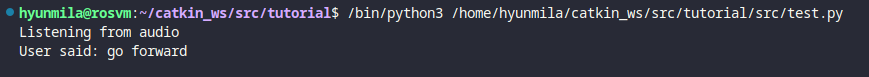
\includegraphics[width=12cm]{files/record.png}
    \captionof{figure}{Wynik funkcji służącej do odczytywania dźwięku z pliku audio.}
    \label{fig:record}
\end{center}

Analogicznie do znajdującej się powyżej, została napisana funkcja odczytująca dane z mikrofonu przy użyciu funkcji \textit{listen} przekazującej wynik do rozpoznania przez Google API \cite{webspeech}.

\begin{lstlisting}[language=Python]
def microphone_recognition():
    r = sr.Recognizer()
    with sr.Microphone() as mic:
        r.adjust_for_ambient_noise(mic)
        audio_data = r.listen(mic, timeout=5)
        query = r.recognize_google(audio_data, language='en-US')
\end{lstlisting}

\begin{center}
    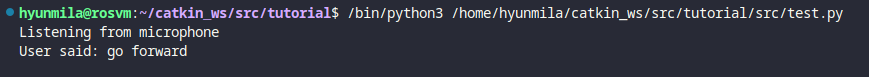
\includegraphics[width=12cm]{files/microphon1.png}
    \captionof{figure}{Wynik funkcji służącej do odczytywania dźwięku z mikrofonu}
    \label{fig:microphone}
\end{center}

Jak można zauważyć na podstawie wyników obu funkcji (\ref{fig:record}, \ref{fig:microphone}), otrzymany został z góry oczekiwany poprawny rezultat rozpoznania mowy. Jednak pomimo swojej wszechstronności zastosowań, biblioteka ta posiada istotne ograniczenia. Używanie któregokolwiek z interfejsów do rozpoznawania mowy wiąże się z potrzebą dostępu do stałego łącza internetowego i posiadania odpowiedniego klucza API. Jedynie dla Google Web Speech API jest on wbudowany, co nie zmienia faktu, że i ta funkcjonalność ma nałożone ograniczenie. Jako zaimplementowana tylko do przeprowadzania testów, w dowolnej chwili może zostać wycofana przez właściciela - Google - co czyni ją nieaplikowalną do celów produkcyjnych. Ponad to, ilość zapytań pod dany klucz API, nawet dla klucza prywatnego, jest odgórnie limitowana, co znacznie utrudnia zastosowanie którejkolwiek z metod poza środowiskiem testowym.

%---------------------------------------------------------------------------

\section{Środowisko lokalne}
\label{sec:srodLocal}

Innym podejściem do rozpoznawania mowy jest wykorzystanie istniejącego lub zbudowanie własnego modelu lokalnie. Istotą każdego algorytmu wykorzystującego uczenie maszynowe są dane, których użyto do jego wytrenowania. Zarówno dla zadania generowania tekstu, klasyfikacji obrazów czy właśnie rozpoznawania mowy, bez podania modelowi odpowiedniego rodzaju danych, nie jest możliwe osiągnięcie rzetelnego rezultatu. 

Głównym z problemów w kwestii dostępności danych do treningu jest różnica pomiędzy ilością danych opisanych etykietami (ang. labelled data), a nieopisanych (ang. unlabelled data). Ich proporcje są zazwyczaj bardzo nierówne - do uczenia na bazie danych audio istnieją tysiące godzin nagrań bez etykiet, w trakcie kiedy tych opisanych etykietami jest często setki razy mniej. 

Jak wspomniano w \ref{subsec:symbolic} język jest rzeczą płynną, ciągle się zmieniającą w zależności od upływu czasu, szerokości i długości geograficznej czy pochodzenia. Dwie osoby mówiące tym samym językiem mogą z perspektywy technicznej używać go zupełnie inaczej modulując tonację, akcent lub dialekt. Fakt ten sprawia, że zadanie znalezienia odpowiedniej ilości danych audio nagrań spełniających wszystkie kryteria każdego języka jest sporym wyzwaniem. Z tego powodu większość zestawów danych opiera się głównie na języku angielskim, używanym przez największą część populacji \cite{mostspoken}. 

Najprostszym rozwiązaniem jest użycie modelu już wytrenowanego, co umożliwia biblioteka \textit{Huggingface transformers} \cite{hf}. Zapewnia ona dostęp do wielu modeli uczenia maszynowego potrafiących rozpoznawać mowę, w tym do modelu \textit{Wav2Vec 2.0} \cite{baevski2020wav2vec} oraz \textit{Whisper} \cite{radford2022robust}.

%---------------------------------------------------------------------------

\subsection{Model Wav2Vec 2.0}
\label{subsec:wav2vec}

Model ten został najpierw wytrenowany na samych danych audio, a następnie dotrenowany za pomocą zestawu danych transkrybcji audio \textit{LibriSpeech} \cite{libri}. Ważną kwestią jest dobrany sposób trenowania, ponieważ autorzy postawili na użycie SSL, czyli samo-nadzorowanego uczenia (ang. self-supervised learning). Jest to metoda lekko odbiegająca od standardowych rozwiązań, bowiem łączy zarówno podejście nadzorowane jak i nienadzorowane. Modelowi przedstawiane są dane wejściowe bez etykiet oraz dane wyjściowe z etykietami. Bazując na tym, po podaniu mu kontekstu ma za zadanie przewidzieć wynik dla danych nieopisanych. 

Dane audio wchodzące do modelu są kodowane przez wielowarstwową konwolucyjną sieć neuronową (ang. CNN - Convolutional Neural Network). Podobnie jak w \textit{Maskowanym Modelowaniu Językowym} (ang. Masked Language Modelling) część danych, będąca uproszczonym modelem danych wejściowych, jest maskowana, a następnie podawana do sieci \textit{transformers}, która tworzy kontekstową reprezentację danych. Model jest następnie trenowany w zadaniu rozróżnienia prawdziwych danych od zakłóceń. 

Użyty w przykładowym algorytmie do rozpoznawania mowy model Wav2Vec to jego wersja dotrenowana na bazie \num{960} godzin audio o częstotliwości \num{16}kHz. Przy użyciu biblioteki \textit{torchaudio} plik audio jest odczytywany a następnie konwertowany do pożądanej przez model częstotliwości. Wektor audio jest następnie przekazywany do procesora modelu i wyciągana jest predykcja podawana do dekodera. Podany do rozpoznania ten sam plik audio, co w przykładzie \ref{sec:srodZdal} jest widoczny na Rys.\ref{fig:wav2vec}.

\begin{lstlisting}
def audio_reco(audio_path):
  speech, sr = torchaudio.load(audio_path)
  resampler = torchaudio.transforms.Resample(sr, 16000)
  speech = resampler(speech)
  input_features = wav2vec2_processor(speech.squeeze(), 
        return_tensors="pt", sampling_rate=16000)
  ...
  predicted_ids = torch.argmax(logits, dim=-1)
  transcription = wav2vec2_processor.batch_decode(predicted_ids)[0]
\end{lstlisting}

\begin{center}
    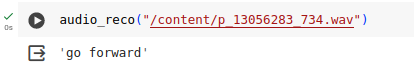
\includegraphics[width=12cm]{files/wav2vectest.png}
    \captionof{figure}{Wynik funkcji służącej do rozpoznawania mowy przy użyciu modelu Wav2Vec}
    \label{fig:wav2vec}
\end{center}

%---------------------------------------------------------------------------

\subsection{Model Whisper}
\label{subsec:whisper}

Drugi z wspomnianych wcześniej modeli rozszerza zakres zastosowań swojego poprzednika dzięki wytrenowaniu za pomocą zestawu danych \num{680,000} godzin zróżnicowanego audio w różnych językach do wykonywania nie tylko rozpoznawania mowy, ale też tłumaczenia, identyfikacji języka i detekcji aktywności głosowej. Dzięki innowatorskiemu podejściu autorów algorytmu, jest w stanie dostosowywać się on do zestawów danych obejmujących szeroki zakres, bez potrzeby dotrenowywania.

W poniższym przykładzie została użyta wersja \textit{medium} modelu, obsługująca wiele języków. Model tak samo jak w powyższym przypadku, przyjmuje dane audio i przetwarza je do częstotliwości \num{16}kHz. Następnie wyciągane są informacje o danych wejściowych i przekazywane do dekodera, który procesuje zadanie transkrybcji w języku angielskim. Otrzymany wynik rozpoznania pliku audio z przykładu \ref{sec:srodZdal} jest widoczny na Rys.\ref{fig:whisper}.

\begin{lstlisting}
def audio_reco(audio_path):
  ...
  forced_decoder_ids = whisper_processor.get_decoder_prompt_ids(
        language="english", task="transcribe")
  predicted_ids = whisper_model.generate(input_features, 
        forced_decoder_ids=forced_decoder_ids)
  transcription = whisper_processor.batch_decode(predicted_ids, 
        skip_special_tokens=True)[0]
\end{lstlisting}

\begin{center}
    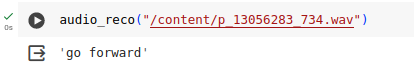
\includegraphics[width=12cm]{files/wav2vectest.png}
    \captionof{figure}{Wynik funkcji służącej do rozpoznawania mowy przy użyciu modelu Whisper}
    \label{fig:whisper}
\end{center}

%---------------------------------------------------------------------------

\section{Ewaluacja}
\label{sec:ewaluacja}

Ewaluacja algorytmów służących do rozpoznawania mowy polega na porównaniu predykcji wykonanej przez model do faktycznej transkrypcji i zapisaniu błędów popełnionych w trakcie zadania. Błędy te można podzielić na trzy kategorie:
\begin{itemize}
    \item zastępstwo (ang. substitution - S) - słowo zostało przetłumaczone w błędny sposób,
    \item dołożenie (ang. insertion - I) - zostało dodane dodatkowe, niewystępujące w nagraniu słowo,
    \item usunięcie (and. deletion - D) - słowo zostało pominięte.
\end{itemize}
Używaną do ewaluacji metryką jest \textit{WER - Word Error Rate}, która liczy błąd na poziomie każdego słowa. Dla audio, w którym wystąpiło N słów, \textit{WER} przedstawia się następująco:
\begin{equation}
    WER = \frac{S+I+D}{N}
\end{equation}

Do ewaluacji został wykorzystany zestaw danych \textit{edinburghcstr/ami} huggingface t\cite{dataset-eval}, składający się ze 100 godzin nagrań spotkań w języku angielskim. Przy użyciu biblioteki \textit{jiwer} \cite{jiwer}, przeprowadzono ewaluację powyższych algorytmów na podstawie zestawu danych \cite{dataset-eval}. Wyniki zostały przedstawione w tabeli \ref{tab:tab1}, gdzie wartość przy nazwie algorytmu jest wartością błędu każdego z nich w skali od 0 do 1.
\begin{table}[h]
    \centering
    \caption{Ewaluacja WER}
    \begin{tabular}{c|c|c}
        Wav2Vec & Whisper & SpeechRecognition  \\ 
        0.736557 & 0.713998 & 0.514967
    \end{tabular}
    \label{tab:tab1}
\end{table}
Oczywiście, wyniki te różnią się znacznie od podanych w pracach na temat wspomnianych powyżej algorytmów wartości zarówno z uwagi na fakt umieszczenia ich w lokalnym środowisku na maszynie bez jednostki obliczeniowej GPU, ale również jakości zestawu danych walidującego poprawność działania. Z uwagi na fakt prostoty w obsłudzie i najniższego współczynnika błędu, w dalszej części pracy jako algorytm będący podstawą działania panelu do sterowania głosowego zostało wybrane podejście zdalne i biblioteka \textit{SpeechRecognition} \cite{speechrec}.
	\chapter{Panel HMI}
\label{cha:panelHmi}

Głównym celem, do którego miało za zadanie prowadzić wybranie odpowiedniego algorytmu uczenia maszynowego do rozpoznawania głosowego było wykonanie panelu HMI. HMI (ang. Human-Machine Interface) jest to z definicji panel służący do połączenia człowieka z urządzeniem lub oprogramowaniem. Pomimo, że pojęcie to określa każdy ekran umożliwiający interakcję z maszyną, jest głównie używane w kontekście przemysłowym do komunikacji ze sterownikami PLC (ang. Programmable Logic Controllers). 
Panel HMI maszyny może być używany między innymi do:
\begin{itemize}
    \item sterowania,
    \item monitorowania wejść i wyjść,
    \item wizualizacji danych,
    \item śledzenia procesów.
\end{itemize}
Panele takie często są budowane do wytrzymywania w ekstremalnych warunkach w zakładach przemysłowych i fabrykach i przystosowywane do działania na odległość. Ich powstanie jest powiązane głównie z potrzebą optymalizacji - dzięki urządzeniom monitorującym procesy zdalnie, pracownicy zakładów zamiast marnować czas na sprawdzanie każdej maszyny po kolei, mogą to zrobić w jednym, dedykowanym do tego miejscu. 

%---------------------------------------------------------------------------

\section{Środowisko pracy}
\label{sec:srodPrac}

Stanowiskiem pracy jest urządzenie z systemem operacyjnym Ubuntu 20.04. W celach użycia narzędzia \textit{Gazebo} \cite{gazebo} służącego do symulowania systemów w czasie rzeczywistym, zainstalowano środowisko \textit{Robot Operating System} (skr.: ROS) \cite{ros}. 

ROS \cite{ros} jest to otwarte oprogramowanie posiadające zestaw bibliotek i narzędzi umożliwiających budowanie aplikacji dla robotów, kompatybilne z językiem programowania \textit{Python}. Dystrybucja zainstalowana na urządzeniu to \textit{ROS Noetic Ninjemys} \cite{noetic}, odmiana dedykowana dla używanego systemu operacyjnego z długoterminowym wsparciem ze strony producenta. 

Do zobrazowania działania algorytmu w symulacji został użyty model TurtleBot3 \cite{turtlebot}. Jest to robot, którego nazwa, wygląd, a nawet sposób poruszania bazuje na Turtle, popularnym robocie będącym integralną częścią języka programowania Logo \cite{logo}. Wybrany model robota to \textit{waffle} (Rys. \ref{fig:gazebo}).

\begin{center}
    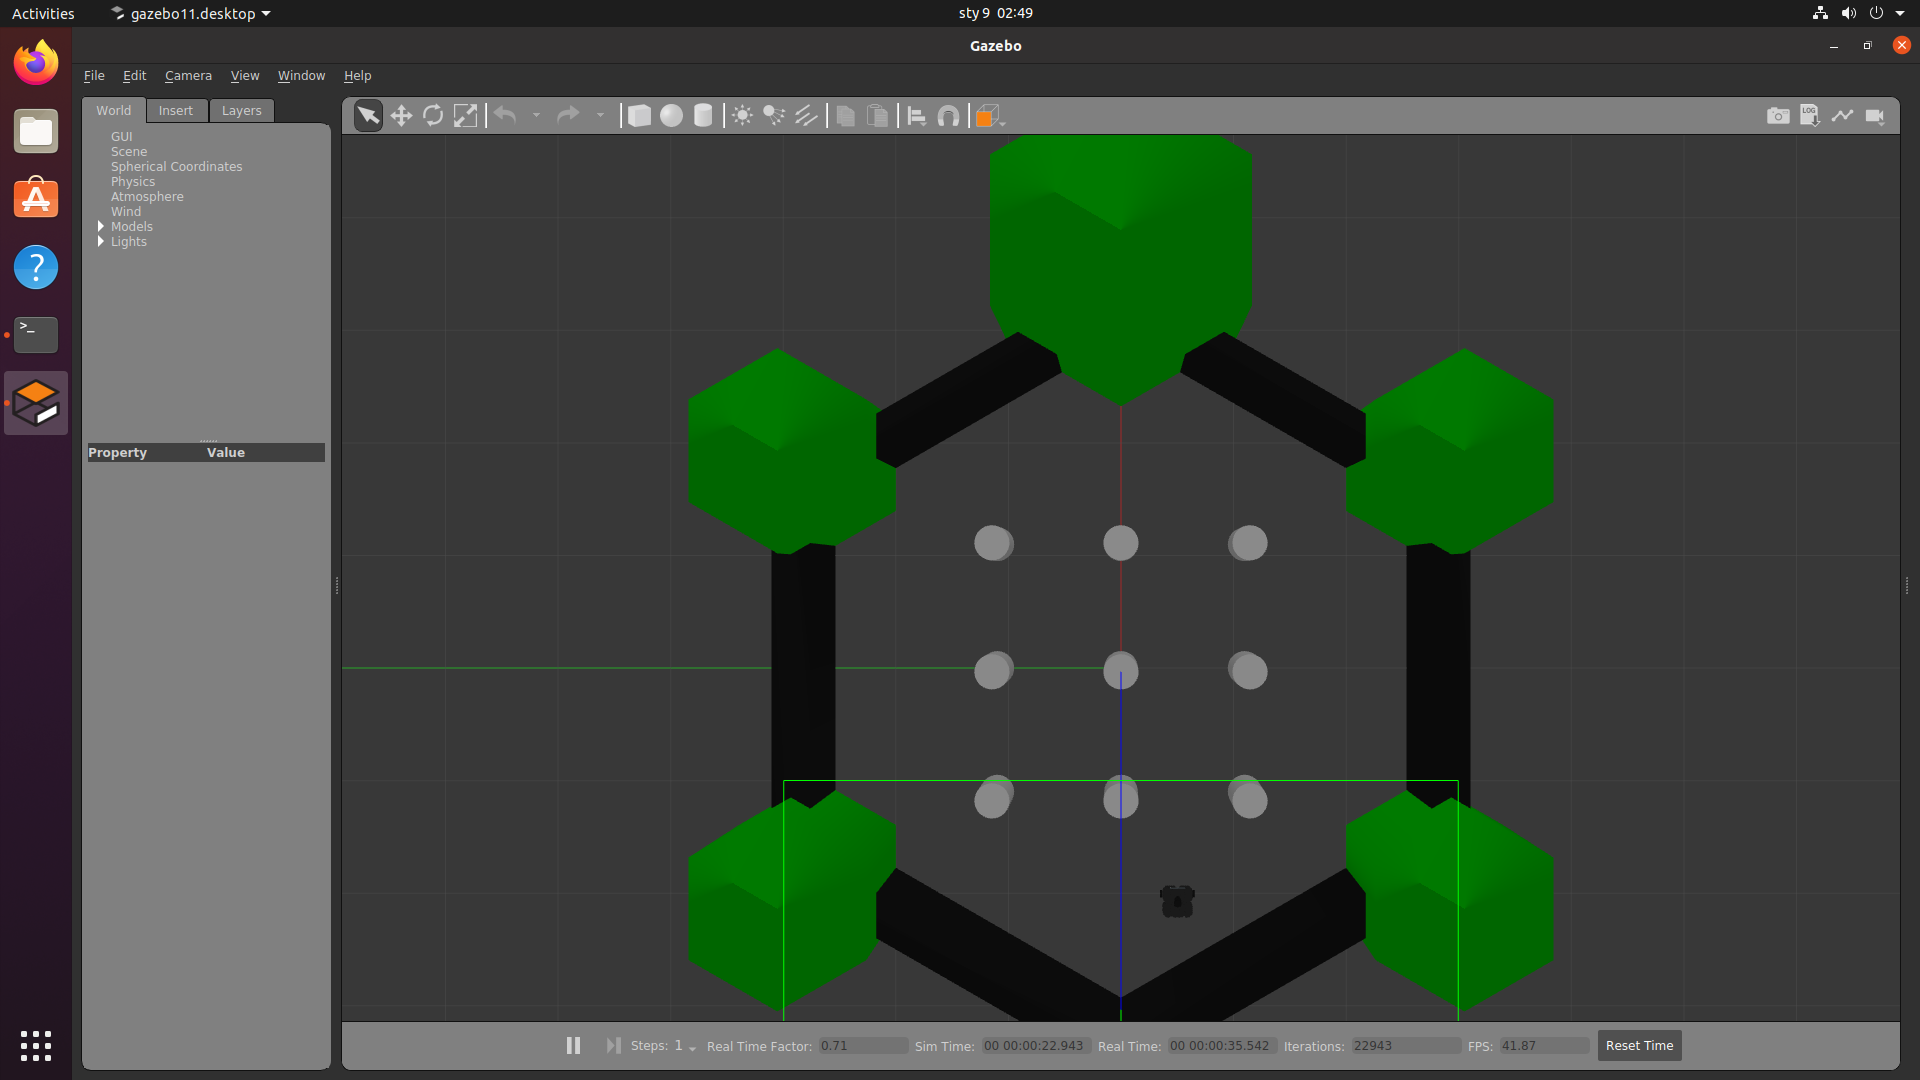
\includegraphics[width=0.8\linewidth]{files/gazebo.png}
    \captionof{figure}{Widok aplikacji Gazebo wraz z uruchomioną symulacją robota.}
    \label{fig:gazebo}
\end{center}

Monitorowanie zaimplementowanego sterowania robotem umożliwia narzędzie \textit{rqt} \cite{rqt}. Jest to oprogramowanie zapewniające szeroki zakres wtyczek do wizualizacji wszelkiego rodzaju danych. Na Rys. \ref{fig:rqt} widoczny jest przykładowy wykres prędkości liniowej kół robota w osi x w czasie. 

\begin{center}
    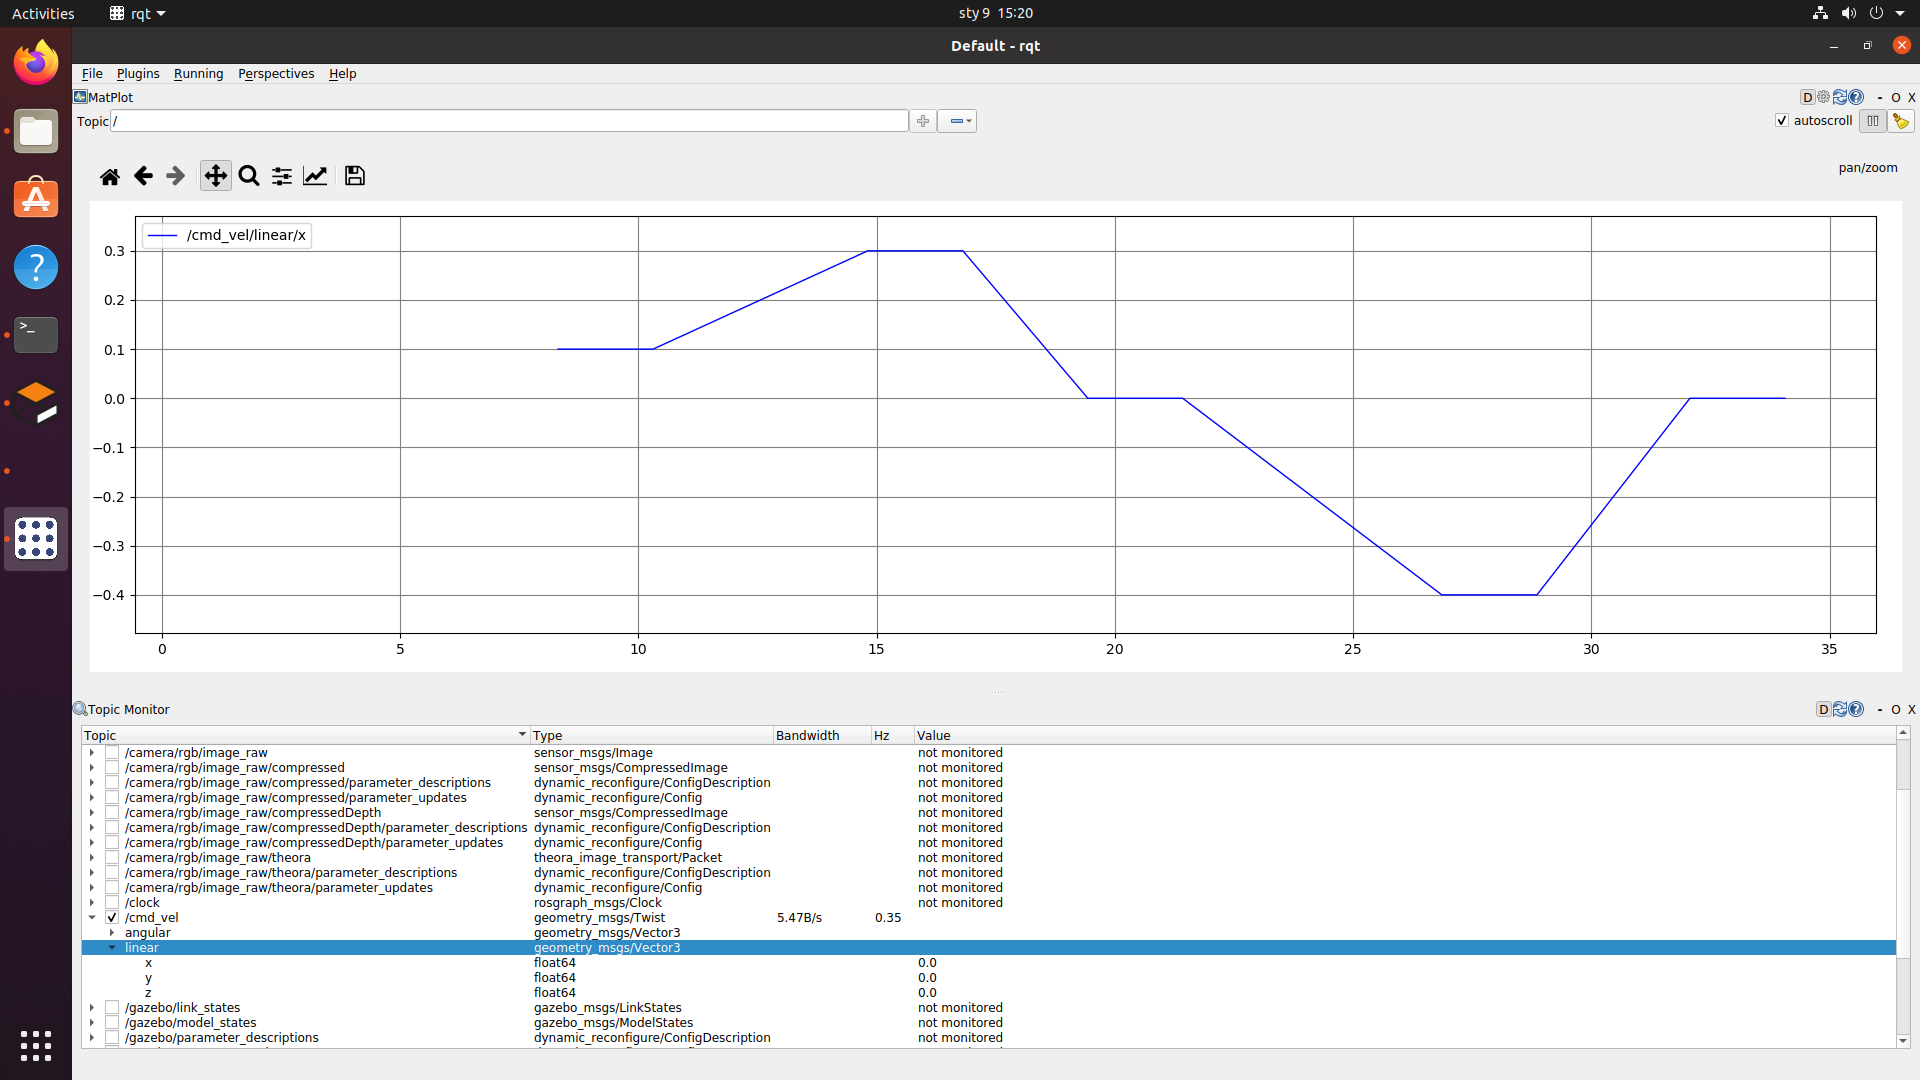
\includegraphics[width=0.8\linewidth]{files/rqt_view.png}
    \captionof{figure}{Widok aplikacji rqt wraz z uruchomioną symulacją poruszania się robota.}
    \label{fig:rqt}
\end{center}

Wymienione powyżej narzędzia służą głównie usprawnieniu pracy w środowisku i weryfikacji założeń projektowych. Sam przebieg działania programu, widoczny na Rys. \ref{fig:diagram} przedstawia się następująco: po starcie programu pojawia się panel do sterowania, który odbiera dane wejściowe audio. Dane te są przekazywane do algorytmu używanego do rozpoznawania mowy, który konwertuje je na komendy. Panel do sterowania przekazuje te komendy robotowi umieszczonemu w symulacji, a ich wykonanie może być odczytane z wykresu.

\begin{center}
    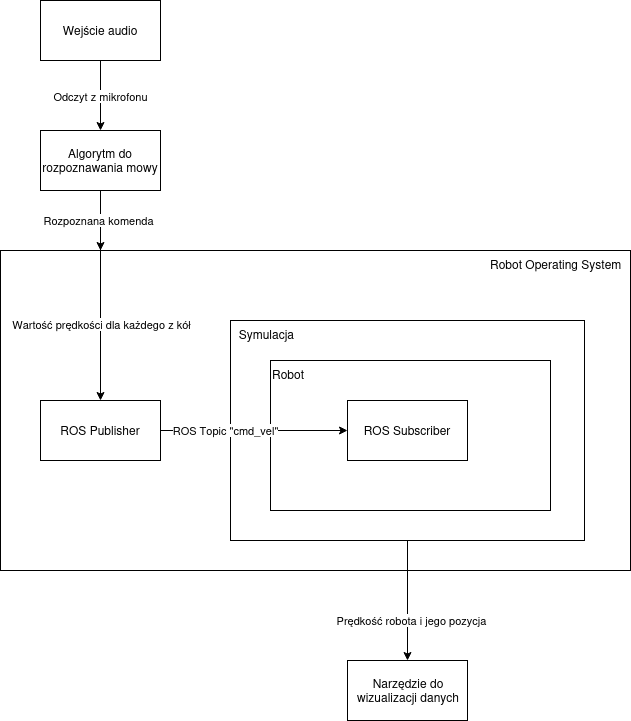
\includegraphics[width=0.95\linewidth]{files/diagram.png}
    \captionof{figure}{Diagram przedstawiający proces działania programu.}
    \label{fig:diagram}
\end{center}

Samo przekazanie przez panel komend robotowi odbywa się za pomocą narzędzia \textit{ROS Topic} (z ang. temat). Tematami w środowisku ROS można określić instancje odpowiedzialne za przekazywanie wiadomości (ang. \textit{messages}) pomiędzy węzłami (ang. \textit{nodes}). Aby nadać jakąś wiadomość na dany temat używany jest \textit{ROS Publisher} (z ang. nadawca). Wiadomość taką może odebrać \textit{ROS Subscriber} (z ang. odbiorca). W widocznym na Rys. \ref{fig:diagram} przebiegu programu, aby umożliwić poruszanie się robota, na temat \textit{cmd-vel}, odpowiedzialny za prędkość kół robota, nadawana jest wiadomość zawierająca pożądaną wartość prędkości kół. Robot, jako subskrybent tego tematu odbiera wiadomość w tym temacie i zaczyna poruszanie się z tą prędkością. 

%---------------------------------------------------------------------------

\section{Aplikacja}
\label{sec:App}

W projekcie w celu wykonania panelu służącego do sterowania głosowego urządzeniem użyto biblioteki dla Pythona \textit{CustomTkinter} \cite{ctk}. Umożliwia ona prostą w obsłudze budowę aplikacji i dostosowanie ich pod potrzeby wizualne użytkownika.

Podstawowym elementem programu jest widoczny na Rys. \ref{fig:panel_1} panel. Przyciski \textit{start} oraz \textit{stop} służą do zmiany stanu robota na ruch lub oczekiwanie. Przy przycisku \textit{start} znajduje się opcjonalne pole służące do wprowadzenia prędkości poruszania się robota. Jest to prędkość liniowa (ang. linear), pozwalająca robotowi na jazdę w przód oraz w tył. Prędkość kątowa (ang. angular) pozwala robotowi na skręcanie w lewo lub w prawo. 
\begin{center}
    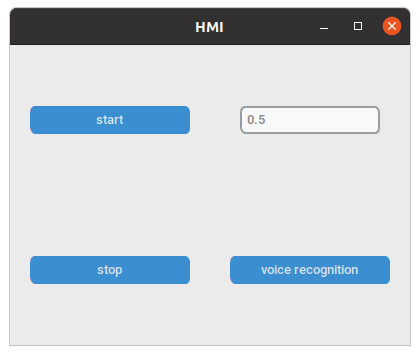
\includegraphics[width=0.8\linewidth]{files/panel_1.png}
    \captionof{figure}{Główne okno panelu HMI.}
    \label{fig:panel_1}
\end{center}

Sterowanie może przebiegać za pomocą zarówno trybu głosowego jak i manualnego. Przycisk \textit{voice recognition} otwiera okno służące do sterowania głosowego. Widoczny na Rys. \ref{fig:panel_2} panel posiada przycik \textit{start/stop speaking} uruchamiający lub zatrzymujący sterowanie głosowe. Ponad to, na polu obok wyświetlane są komendy programu w czasie rzeczywistym.

\begin{center}
    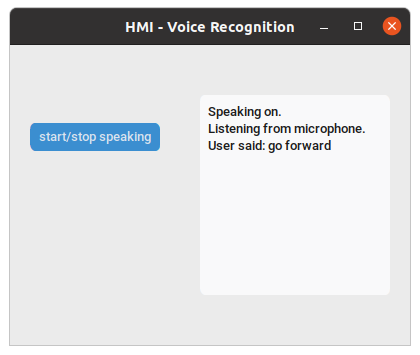
\includegraphics[width=0.8\linewidth]{files/panel_2.png}
    \captionof{figure}{Okno panelu HMI służące do sterowania głosowego.}
    \label{fig:panel_2}
\end{center}

\break
Monitorowanie sterowania robotem jest możliwe dzięki wykorzystaniu wspomnianego wcześniej narzędzia \textit{rqt} \cite{rqt}. Na Rys. \ref{fig:rqt2} widoczny jest wykres wiadomości publikowanych przez robota w temacie \textit{cmd-vel} o jego prędkości liniowej w osi x.

\begin{center}
    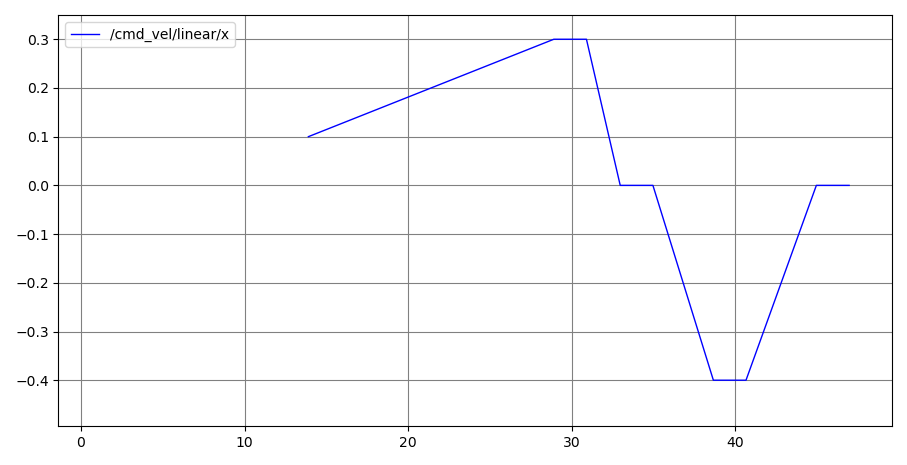
\includegraphics[width=0.9\linewidth]{files/rqt2.png}
    \captionof{figure}{Prędkość liniowa robota w czasie.}
    \label{fig:rqt2}
\end{center}

Natomiast z wykresu widocznego na Rys. \ref{fig:rqt3} można odczytać wartości publikowane przez symulację w temacie \textit{pose}, informującym o pozycji robota.

\begin{center}
    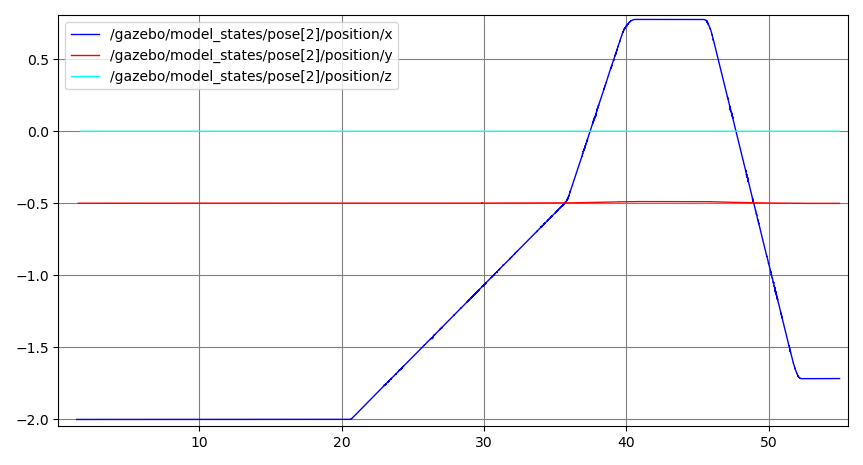
\includegraphics[width=0.9\linewidth]{files/rqt3.png}
    \captionof{figure}{Pozycja robota w symulacji w czasie.}
    \label{fig:rqt3}
\end{center}
	\chapter{Testy}
\label{cha:testy}

Sterowanie za pomocą komend głosowych może stać się o wiele cięższe w wykonaniu, kiedy w grę wchodzą czynniki takie jak akcent, inny niż stosowany w algorytmie język, dźwięki w tle, złożoność polecenia czy nawet niewyraźna mowa. Z uwagi na ten fakt, algorytm do rozpoznawania mowy używany w programie został poddany scenariuszom testowym. 

Na potrzeby testów stworzono pięć zestawów tych samych dziesięciu poleceń, różniących się pomiędzy sobą kilkoma czynnikami:
\begin{itemize}
    \item oryginalny zestaw komend w języku angielskim z akcentem amerykańskim \textit{[EN]},
    \item wersja w języku angielskim z akcentem amerykańskim, gdzie prędkość nagrania to 2.0 \textit{[EN-0-2]},
    \item wersja w języku angielskim z akcentem Indii \textit{[EN-IN]},
    \item wersja w języku angielskim z akcentem Hong Kongu, gdzie prędkość nagrania to 0.5, a tonacja wyższa o 20 od normalnej \textit{[EN-HK-20-05]},
    \item wersja w języku polskim \textit{[PL]}.
\end{itemize}

Do zestawów danych została dołożona również wersja polska, celem sprawdzenia użyteczności algorytmu w wypadku implementacji na fizycznym urządzeniu. Modyfikacje prędkości, tonacji i akcentów zostały wykonane na potrzeby zróżnicowania danych i wprowadzenia trudności dla algorytmu do zrozumienia komend. 

Używając metryki WER \ref{eq:wer} została obliczona średnia wartość błędu w skali od 0 do 1 dla każdego z zestawów danych, widoczna na wykresie \ref{fig:dts1}. Można na nim zauważyć, że zgodnie z oczekiwaniami, zestaw \textit{[EN]} oryginalnych komend w języku angielskim posiada najmniejszą wartość błędu. Zarówno zestaw z akcentem Indii \textit{[EN-IN]} jak ten z akcentem Hong Kongu radzą sobie równie dobrze. Najbardziej wyróżnia się zestaw komend po polsku \textit{[PL]}, ze względu na niewystępujące w transkrypcji znaki łacińskie.

\begin{center}
    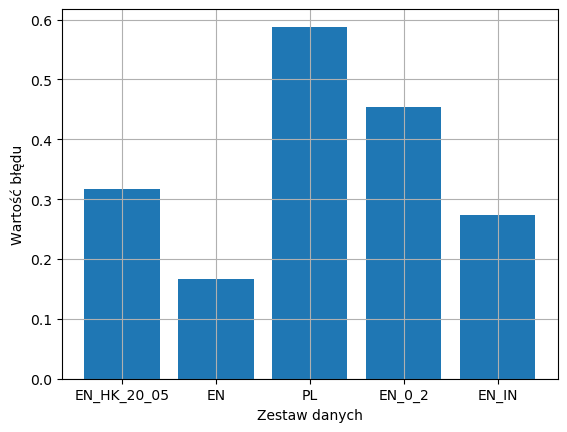
\includegraphics[width=0.7\linewidth]{files/output1.png}
    \captionof{figure}{Średnia wartość błędu}
    \label{fig:dts1}
\end{center}

Po uwzględnieniu w transkrypcji znaków łacińskich, można zauważyć na wykresie \ref{fig:dts2} znaczny spadek wartości błędu dla zestawu komend w języku polskim. Potwierdza to użyteczność wykorzystywanego algorytmu do rozpoznawania mowy również poza środowiskiem testowym.

\begin{center}
    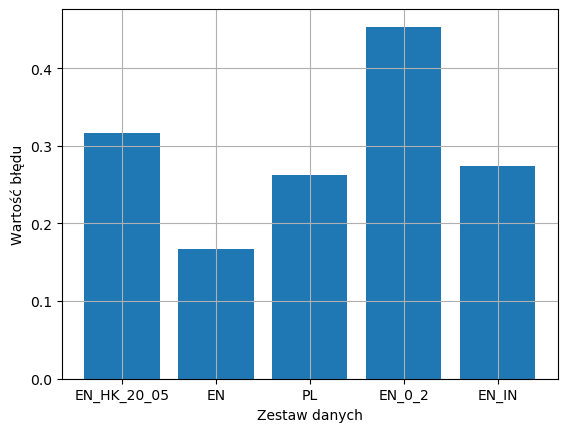
\includegraphics[width=0.7\linewidth]{files/output2.png}
    \captionof{figure}{Średnia wartość błędu po uwzględnieniu znaków łacińskich}
    \label{fig:dts2}
\end{center}

Dane w zestawach dzielą się na dwie kategorie pod względem długości polecenia:
\begin{itemize}
    \item proste komendy poniżej 15 znaków \textit{[słowa krótkie]},
    \item bardziej złożone komendy powyżej 15 znaków \textit{[słowa długie]}.
\end{itemize}

% dopisz tu cos TODO
% czy dodawac reference  do stronki konwertera

\begin{center}
    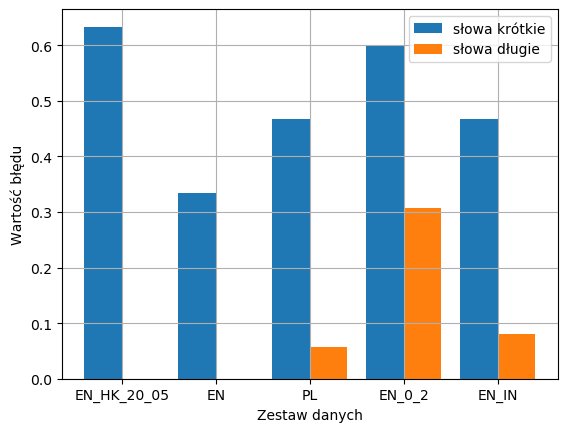
\includegraphics[width=0.7\linewidth]{files/output3.png}
    \captionof{figure}{Średnia wartość błędu dla słów krótkich i słów długich}
    \label{fig:dts3}
\end{center}

%  jeszcze wykres x to slowa y to srednie rozpoznawanie ich? - nwm zobacze rano
% analiza tych zestawow danych, gdzie jest modyfikacja - WAZNE
% tutaj jeszcze mozna wrzucic testy samego robota - nie wiem jeszcze jak

% Scenariusze testowe:
% 1. inny akcent niz eng-us - indi
% 1. mowa po polsku - czy w ogole rozpoznaje język?
% 2. złożone komendy
% 3. muzyka np w tle/bardzo cicho
% chin - pitch -20, speed -0.5
% indi - speed 2.0

%---------------------------------------------------------------------------
    \chapter{Podsumowanie}
\label{cha:podsumowanie}

% wykonanie panelu bylo troche ciezkie w kontekscie doboru narzędzi
%  dużo czasu zajęło przeprowadzenie ewaluacji algorytmow 
% to co jest uzywane do rozpoznawania glosowego niekoniecznie dziala idealnie - jak widac na wykresach

%---------------------------------------------------------------------------
	
	% itd.
	% \appendix
	% \include{dodatekA}
	% \include{dodatekB}
	% itd.
	
	\printbibliography

\end{document}
